\documentclass{article}
\usepackage[bottom=0.5cm, right=1.5cm, left=1.5cm, top=1.5cm]{geometry}
\usepackage{amsmath}
\usepackage{amssymb}
\usepackage{amsthm}
\usepackage{enumitem}
\usepackage{exercise} % Exercises Style
\usepackage{graphicx}
\usepackage{caption}
\usepackage{environ}
\newenvironment{solution}
  {\renewcommand\qedsymbol{$\blacksquare$}\begin{proof}[Solution]$ $}
  {\end{proof}}



% Enable Code
\usepackage{minted}
\let \extra T

\newcommand{\vect}[1]{\boldsymbol{#1}}
\DeclareMathOperator{\Tr}{Tr}
\DeclareMathOperator{\Cov}{Cov}
\DeclareMathOperator{\Var}{Var}
\DeclareMathOperator{\E}{E}


\title{Solutions to Assignment 1}
\author{Rongfei Jin}
\begin{document}
\maketitle


\begin{Exercise}
    \begin{solution}
        The minimization is found by differentiation,
        \[
            d(\sum_{j=1}^{n}(X_j -\theta)^2) = \sum_{j=1}^{n} -2X_j + 2\theta = -2(\sum_{j=1}^{n}X_j - \sum_{j=1}^{n}\theta)
        \]

        We check that the point is indeed a minima by deriving the 2nd derivative
        \[
            d^2(\sum_{j=1}^{n}(X_j -\theta)^2) = 2n>0
        \]

        We set the gradient to 0 and get the \(\theta\) that minimize the expression

        \begin{align*}
            \sum_{j=1}^{n}\theta & = \sum_{j=1}^{n}X_j            \\
            \hat \theta          & = \frac{1}{n}\sum_{j=1}^{n}X_j
        \end{align*}

        For part 2, we note that \[|X_j - \eta| = \begin{cases}
                X_j - \eta   & \text{if } X_j >= \eta \\
                - X_j + \eta & \text{if } X_j < \eta  \\
            \end{cases}\]

        Now we define the order statistics by sorting the realization value of \(X_1, X_2,\ldots, X_n\) in increasing order as such

        \[X_{(1)}, X_{(2)}, \ldots, X_{(n)}\] where \(X_{(1)} \le X_{(2)} \le \ldots \le X_{(n)}\)

        When \(n\) is even
        Let \(k\in \mathbb Z^+\) such that \(X_{(k)} \le \eta \le X_{(k+1)}\) where \(0<k<n\)

        \begin{align*}
            \underset{\eta\in \mathbb R}{\arg\min}\sum_{j=1}^{n}|X_j - \eta|
             & = \underset{\eta\in \mathbb R, k\in \mathbb Z^+}{\arg\min}(\sum_{j=1}^{k}(- X_{(j)} + \eta) + \sum_{j=k+1}^{n}(X_{(j)} - \eta))      \\
             & = \underset{\eta\in \mathbb R, k\in \mathbb Z^+}{\arg\min}\sum_{j=1}^{k} (-X_{(j)}) + \sum_{j=k+1}^{n}(X_{(j)})+ (k-(n-(k+1)+1))\eta \\
             & =\underset{\eta\in \mathbb R, k\in \mathbb Z^+}{\arg\min} \sum_{j=1}^{k} (-X_{(j)}) + \sum_{j=k+1}^{n}(X_{(j)})+ (2k-n)\eta          \\
             & =\underset{\eta\in \mathbb R, k\in \mathbb Z^+}{\arg\min} (2k-n)\eta
        \end{align*}

        Now we differentiate and find the minima
        \[\frac{\partial}{\partial \eta}((2k-n)\eta) = 2k-n\]
        \[k = n/2\]

        if \(n\) is even, then we can let \(k=n/2\)
        However, if \(n\) is odd, then the minima \(n/2\) is not defined, therefore, we must find the next best value.

        Since \(n\) is odd, we let \(n=2m-1\) where \(m\) is any positive integer, if \(k>m\) then \(2k-n > 2m - (2m-1) = 1\), if \(k\le m-1\) then \(2k-n \le 2m - 2 - (2m-1) = -1\), therefore, the best \(k\) must be in the range \(m-1 < k \le m\), and the only possible value is \(k=m\) since \(m\) is only integer in this range


        we found that the change of the expression with respect to \(\eta\) is constant, which means the order which \(\eta\) locates in the sequenence \(A_j\) matters rather that the value of \(\eta\).

        The expression \(\sum_{j=1}^{n}|A_j -\eta|\) is minimized when \(k=n/2\) if \(n\) is even and \(k=(n+1)/2\) if \(n\) is odd, which means \(\hat \eta = \text{median of }A_j\)
    \end{solution}
\end{Exercise}
\pagebreak
% Exercise 2
\begin{Exercise}
    \begin{solution}
        \begin{align*}
            \Cov(X,Y) & = \E((X-E(X))(Y-E(Y))                                                                      \\
                      & = E(XY - XE(Y) - XE(Y)+E(X)E(Y))                                                           \\
                      & = E(XY) - E(XE(Y)) - E(XE(Y))+E(E(X)E(Y)) & \text{(Expectation Linearity)\cite{wasserman}} \\
                      & = E(XY) - E(X)E(Y)                                                                         \\
        \end{align*}
    \end{solution}
\end{Exercise}
\pagebreak
% Exercise 3
\begin{Exercise}
    \begin{solution}

        \[
            L(\lambda|x_1, x_2, \ldots, x_n) = \prod_{i=1}^{n}\lambda e^{-\lambda x_i}
        \]

        \begin{align*}
            l(\lambda|x_1, x_2, \ldots, x_n) & = \log(\prod_{i=1}^{n}\lambda e^{-\lambda x_i}) \\
                                             & = \sum_{i=1}^{n}\log(\lambda) + (-\lambda x_i)  \\
                                             & = n\log(\lambda) - \lambda\sum_{i=1}^{n}x_i     \\
        \end{align*}

        \begin{align*}
            \frac{\partial}{\partial \lambda}(n\log(\lambda) - \lambda\sum_{i=1}^{n}x_i)
             & = \frac{n}{\lambda} - \sum_{i=1}^{n} x_i                                     \\
            \frac{\partial}{\partial^2 \lambda}(n\log(\lambda) - \lambda\sum_{i=1}^{n}x_i)
             & = -\frac{n}{\lambda^2} < 0               & \text{(The point is the maximum)}
        \end{align*}

        \begin{align*}
            \frac{\partial}{\partial \lambda}      & = 0 \\
            \frac{n}{\lambda} - \sum_{i=1}^{n} x_i & = 0 \\
        \end{align*}

        \[\hat \lambda                           = \frac{n}{\sum_{i=1}^{n}x_i}\]
    \end{solution}
\end{Exercise}
\pagebreak
% Exercise 4
\begin{Exercise}
    \begin{solution}
        \begin{align*}
            L(\vect{\mu}; \vect{\vect{\Sigma}}|\vect{x_1},\ldots,\vect{x_n}) & = \prod_{i=1}^{n}\frac{1}{2\pi|\vect{\Sigma}|^{1/2}}\exp\{-\frac{1}{2} (\vect{x}_i-\vect{\mu})^T \vect{\Sigma}^{-1} (\vect {x_i} -\vect \mu)\}                                                                            \\
            l(\vect{\mu}; \vect{\vect{\Sigma}}|\vect{x_1},\ldots,\vect{x_n}) & = \log(\prod_{i=1}^{n}\frac{1}{2\pi|\vect{\Sigma}|^{1/2}}\exp\{-\frac{1}{2} (\vect{x}_i-\vect{\mu})^T \vect{\Sigma}^{-1} (\vect{x}_i -\vect \mu)\})                                                                       \\
            l(\vect{\mu}; \vect{\vect{\Sigma}}|\vect{x_1},\ldots,\vect{x_n}) & = n \log(\frac{1}{2\pi|\vect{\Sigma}|^{1/2}})-\frac{1}{2}\sum_{i=1}^n ((\vect{x}_i-\vect{\mu})^T \vect{\Sigma}^{-1} (\vect{x}_i -\vect \mu))                                                                              \\
            l(\vect{\mu}; \vect{\vect{\Sigma}}|\vect{x_1},\ldots,\vect{x_n}) & = n \log(\frac{1}{2\pi|\vect{\Sigma}|^{1/2}})-\frac{1}{2}\sum_{i=1}^n (\vect {x_i}^T\vect{\Sigma}^{-1}\vect{x}_i - 2\vect{x}_i^T\vect{\Sigma}^{-1}\vect{\mu} + \vect{\mu}^T \vect{\Sigma}^{-1}\vect{\mu})                 \\
                                                                             & \text{(}\vect{x}_i^T \vect{\Sigma}^{-1}\vect{\mu}, \vect{\mu}_i^T \vect{\Sigma}^{-1}\vect{x},\text{ are scalars, so they're the same}\text{)}                                                                             \\
            l(\vect{\mu}; \vect{\vect{\Sigma}}|\vect{x_1},\ldots,\vect{x_n}) & = n \log(\frac{1}{2\pi|\vect{\Sigma}|^{1/2}})+\sum_{i=1}^n (-\frac{1}{2}\vect {x_i}^T\vect{\Sigma}^{-1}\vect{x}_i + \vect{x}_i^T\vect{\Sigma}^{-1}\vect{\mu} - \frac{1}{2} \vect{\mu}^T \vect{\Sigma}^{-1}\vect{\mu})     \\
            l(\vect{\mu}; \vect{\vect{\Sigma}}|\vect{x_1},\ldots,\vect{x_n}) & = -n\log(2\pi) - \frac{n}{2}\log(\vect{|\Sigma}|)+\sum_{i=1}^n (-\frac{1}{2}\vect {x_i}^T\vect{\Sigma}^{-1}\vect{x}_i + \vect{x}_i^T\vect{\Sigma}^{-1}\vect{\mu} - \frac{1}{2} \vect{\mu}^T \vect{\Sigma}^{-1}\vect{\mu}) \\
        \end{align*}

        \begin{align*}
            \frac{\partial}{\partial \vect \mu} & = \sum_{i=1}^n \vect{x}_i^T \vect{\Sigma}^{-1} - \sum \vect \mu^T \vect \Sigma^{-1} \\
                                                & = \sum_{i=1}^n \vect{x}_i^T \vect{\Sigma}^{-1} - n \vect \mu^T \vect \Sigma^{-1}    \\
        \end{align*}

        \begin{align*}
            n \vect \mu^T \vect \Sigma^{-1}                            & = \sum_{i=1}^n \vect{x}_i^T \vect{\Sigma}^{-1} & \text{(Set gradient to 0)}                  \\
            n \vect \Sigma^{-1} \vect \mu                              & = \vect{\Sigma}^{-1} \sum_{i=1}^n \vect{x}_i   & \text{(Note that co-variance is symmetric)} \\
            \vect \mu                                                  & = \overline{\vect{x}_i}                                                                      \\
            \hat {\vect \mu}                                           & = \begin{pmatrix}
                                                                               \overline{x_{1i}} \\
                                                                               \overline{x_{2i}}
                                                                           \end{pmatrix}                                                   \\
            \begin{pmatrix} \hat {\mu}_1 \\ \hat {\mu}_2 \end{pmatrix} & = \begin{pmatrix}
                                                                               \frac{1}{n} \sum_{i=1}^{n} x_{i1} \\
                                                                               \frac{1}{n} \sum_{i=1}^{n}  x_{i2}
                                                                           \end{pmatrix}
        \end{align*}

        We break down the partial differentiation of \(\Sigma^{-1}\) into 2 parts,
        \begin{align*}
            \frac{\partial}{\partial \vect \Sigma^{-1}}(-\frac{n}{2}\log (|\vect{\Sigma}|))
             & = \frac{\partial}{\partial \vect \Sigma^{-1}}(\frac{n}{2}\log (|\vect{\Sigma}^{-1}|))                                              \\
             & = \frac{n}{2}\frac{1}{|\vect{\Sigma}^{-1}|}|\vect{\Sigma}^{-1}|(\vect{\Sigma})^T      & \text{Determinant Derivative}\cite{matrix} \\
             & = \frac{n}{2}\vect{\Sigma}                                                                                                         \\
        \end{align*}
        \begin{align*}
            \frac{\partial}{\partial \vect{\Sigma}}(-\frac{1}{2}\sum_{i=1}^n ((\vect{x}_i-\vect{\mu})^T \vect{\Sigma}^{-1} (\vect{x}_i -\vect \mu)))
             & = -\frac{1}{2} \frac{\partial}{\partial \vect{\Sigma}} \sum_{i=1}^n \Tr((\vect{x}_i-\vect{\mu}) (\vect{x}_i -\vect \mu)^T \vect{\Sigma}^{-1}) \\
             & = -\frac{1}{2} \sum_{i=1}^n \Tr((\vect{x}_i-\vect{\mu}) (\vect{x}_i -\vect \mu)^T)                                                            \\
             & = -\frac{1}{2} \sum_{i=1}^n ((\vect{x}_i-\vect{\mu}) (\vect{x}_i -\vect \mu)^T)
        \end{align*}

        We then add part 1 and 2 together and set this gradient to 0
        \[
            \frac{n}{2}\vect{\Sigma} - \frac{1}{2} \sum_{i=1}^n ((\vect{x}_i-\vect{\mu})(\vect{x}_i -\vect \mu)^T) = 0
        \]
        \begin{align*}
            \vect{\Sigma} & = \frac{\sum_{i=1}^n ((\vect{x}_i-\vect{\mu})(\vect{x}_i -\vect \mu)^T)}{n}                                               \\
                          & = \frac{1}{n}\sum_{i=1}^n (\vect x_i \vect x_i^T - \vect x_i \vect \mu^T - \vect \mu \vect x_i^T + \vect \mu \vect \mu^T) \\
                          & = \frac{1}{n} \sum_{i=1}^{n}
            \begin{pmatrix}x_{i1} \\ x_{i2}\end{pmatrix}\begin{pmatrix}x_{i1} & x_{i2}\end{pmatrix}
            - \begin{pmatrix}x_{i1} \\ x_{i2}\end{pmatrix}\begin{pmatrix}\mu_{1} & \mu_{2}\end{pmatrix}
            - \begin{pmatrix}\mu_{1} \\ \mu_{2}\end{pmatrix}\begin{pmatrix}x_{i1} & x_{i2}\end{pmatrix}
            + \begin{pmatrix}\mu_{1} \\ \mu_{2}\end{pmatrix}\begin{pmatrix}\mu_{1} & \mu_{i2}\end{pmatrix}                                            \\
                          & = \frac{1}{n} \sum_{i=1}^{n}
            \begin{pmatrix}x_{i1}^2 & x_{i1}x_{i2} \\ x_{i1} x_{i2} & x_{i2}^2\end{pmatrix}
            - \begin{pmatrix}x_{i1}\mu_{1} & x_{i1}\mu_{2} \\ x_{i2} \mu_1 & x_{i2} \mu_2\end{pmatrix}
            - \begin{pmatrix}x_{i1}\mu_{1} & x_{i2}\mu_{1} \\ x_{i1} \mu_2 & x_{i2} \mu_2\end{pmatrix}
            + \begin{pmatrix}\mu_{1}^2 & \mu_{1}\mu_{2} \\ \mu_{1} \mu_{i2} & \mu_{2}^2\end{pmatrix}                                                  \\
                          & = \frac{1}{n} \sum_{i=1}^{n}
            \begin{pmatrix}
                x_{1i}^2 - 2x_{i1} \mu_1 + \mu_1^2                         & x_{i1}x_{i2} - x_{i1} \mu_2 - x_{i2} \mu_{1} + \mu_1 \mu_2 \\
                x_{i1}x_{i2} - x_{i1} \mu_2 - x_{i2} \mu_{1} + \mu_1 \mu_2 & x_{2i}^2 - 2x_{i1} \mu_2 + \mu_2^2
            \end{pmatrix}                   \\
                          & = \frac{1}{n} \sum_{i=1}^{n}
            \begin{pmatrix}
                (x_{i1} - \mu_1)^2               & (x_{i1} - \mu_1)(x_{i2} - \mu_2) \\
                (x_{i1} - \mu_1)(x_{i2} - \mu_2) & (x_{i2} - \mu_2)^2               \\
            \end{pmatrix}                                                                       \\
                          & =
            \begin{pmatrix}
                \frac{1}{n} \sum_{i=1}^{n} (x_{i1} - \mu_1)^2 &
                \frac{1}{n} \sum_{i=1}^{n} (x_{i1} - \mu_1)(x_{i2} - \mu_2)                                   \\
                \frac{1}{n} \sum_{i=1}^{n} (x_{i1} - \mu_1)(x_{i2} - \mu_2)
                                                              & \frac{1}{n} \sum_{i=1}^{n} (x_{i2} - \mu_2)^2 \\
            \end{pmatrix}
        \end{align*}

        \begin{align*}
            \frac{1}{n} \sum_{i=1}^{n} (x_{i1} - \mu_1)(x_{i2} - \mu_2) & =
            \frac{1}{n} \frac{\sum_{i=1}^{n} (x_{i1} - \mu_1)(x_{i2} - \mu_2)}{\sqrt{\sum_{i=1}^{n} (x_{i1} - \mu_1)^2 \cdot \sum_{i=1}^{n} (x_{i2} - \mu_2)^2}} \sqrt{\sum_{i=1}^{n} (x_{i1} - \mu_1)^2 \cdot \sum_{i=1}^{n} (x_{i2} - \mu_2)^2}
        \end{align*}

        Now it is clear that we have the following estimation:

        \[\hat{\sigma}_1^2 = \frac{1}{n} \sum_{i=1}^{n} (x_{i1} - \mu_1)^2 \]
        \[\hat{\sigma}_2^2 = \frac{1}{n} \sum_{i=1}^{n} (x_{i2} - \mu_2)^2 \]
        \[\hat \rho = \frac{1}{\sqrt{\hat \sigma_1 \hat \sigma_2}}\frac{1}{n} \sum_{i=1}^{n} (x_{i1} - \mu_1)(x_{i2} - \mu_2)\]
    \end{solution}
\end{Exercise}
\pagebreak
\begin{Exercise}
    \begin{solution}
        \begin{enumerate}[label=(\roman*)]
            \item
                  %Code
                  \ifx \extra T
                      \begin{minted}{R}
generate_n_gamma <- function(n, alpha=1, beta=1) {
  delta = 1/beta
  
  gammas <- c() 
  for (i in 1:n) {
    us <- sample.int(.Machine$integer.max, size = alpha, replace=TRUE)
    us <- us / .Machine$integer.max
    exp <- -log(us) / delta
    gammas <- c(gammas,sum(exp))
  }
  return (gammas)
}
            \end{minted}
                  \fi
            \item
                  \begin{align*}
                      L(\alpha, \beta| x_1,x_2,\ldots,x_n) & = \prod_{i=1}^{n}\frac{1}{\Gamma(\alpha)\beta^{\alpha}}x^{\alpha-1}e^{-\frac{x}{\beta}}       \\
                      l(\alpha, \beta| x_1,x_2,\ldots,x_n) & = \log(\prod_{i=1}^{n}\frac{1}{\Gamma(\alpha)\beta^{\alpha}}x^{\alpha-1}e^{-\frac{x}{\beta}}) \\
                      l(\alpha, \beta| x_1,x_2,\ldots,x_n) & = \sum_{i=1}^{n}-\log(\Gamma(\alpha))-a\log\beta+(\alpha-1)\log(x_i)-\frac{x_i}{\beta}        \\
                      l(\alpha, \beta| x_1,x_2,\ldots,x_n) & = -n\log(\Gamma(\alpha))-n\cdot a\log\beta
                      +(\alpha-1)\sum_{i=1}^{n}\log(x_i)-\frac{1}{\beta}\sum_{i=1}^{n}x_i                                                                  \\
                  \end{align*}

                  \begin{align*}
                      \frac{\partial}{\partial \beta}(l(\alpha, \beta| x_1,x_2,\ldots,x_n))  = -\frac{n\alpha}{\beta}+\frac{1}{\beta^2} \sum_{i=1}^{n} x_i
                  \end{align*}

                  \begin{align*}
                      \frac{\partial}{\partial \beta}(l(\alpha, \beta| x_1,x_2,\ldots,x_n)) & = 0 \\
                      -\frac{n\alpha}{\beta}+\frac{1}{\beta^2} \sum_{i=1}^{n} x_i           & = 0 \\
                  \end{align*}
                  \[\hat \beta = \frac{\sum_{i=1}^{n}x_i}{na} = \frac{\bar x}{a}\]

                  \begin{align*}
                      l(\alpha, \beta| x_1,x_2,\ldots,x_n) & =
                      -n\log(\Gamma(\alpha))
                      -n\cdot a(\log(\bar x) - \log(\alpha))
                      + (\alpha-1)\sum_{i=1}^{n}\log(x_i)-
                      \frac{a}{\bar x}\sum_{i=1}^{n}x_i        \\
                                                           & =
                      -n\log(\Gamma(\alpha))
                      -na\log(\bar x) +na\log(\alpha)
                      + \alpha\sum_{i=1}^{n}\log(x_i) - \sum_{i=1}^{n}\log(x_i)
                      - an
                  \end{align*}
                  Note that we define \(\psi(\alpha) = \frac{\Gamma'(\alpha)}{\Gamma(\alpha)}\)
                  \begin{align*}
                      \frac{\partial}{\partial \alpha} l(\alpha, \beta| x_1,x_2,\ldots,x_n)
                                   & = -n\frac{1}{\Gamma(\alpha)}\Gamma(\alpha)\psi(\alpha) + - n\log(\bar x) + n(\log(\alpha)+1) + \sum_{i=1}^{n}\log(x_i) - n \\
                                   & = -n\psi(\alpha) + - n\log(\bar x) + n\log(\alpha) + \sum_{i=1}^{n}\log(x_i)                                               \\
                      \psi(\alpha) & = - \log(\bar x) + \log(\alpha) + \frac{1}{n}\sum_{i=1}^{n}\log(x_i)                                                       \\
                  \end{align*}
                  %Code
                  \ifx \extra T
            \item
                  \begin{minted}{R}
d <- function(f, x, h = 1e-7) {
  (f(x + h) - f(x - h)) / (2*h)
}

newton <- function(f, x0, tol = 1e-9, maxiter = 100) {
  x <- x0
  for (i in seq_len(maxiter)) {
    fx <- f(x)
    dfx <- d(f, x)
    
    if (abs(dfx) < 1e-15) {
      stop("Numerical derivative too small. Unable to proceed")
    }
    
    x_new <- x - fx / dfx
    
    if (abs(x_new - x) < tol) {
      return(x_new)
    }
    x <- x_new
  }
  stop("Max iterations reached without convergence")
}

mle_gamma <- function(xs){
  n <- length(xs)
  x_bar <- mean(xs)
  log_x_bar <- mean(log(xs))
  f <- function(alpha) log(alpha) - digamma(alpha) - (log(x_bar) - log_x_bar)
  a <- newton(f, 1)
  return (c(a, x_bar/a))
} 
                  \end{minted}
            \item
                  \begin{minted}{R}
n_arr <- seq(10,2000,10)
true_alpha <- 10
true_beta <- 5
abs_diff_alpha = c()
abs_diff_beta = c()
for (n in n_arr) {
    x <- generate_n_gamma(n, true_alpha, true_beta)
    hats <- mle_gamma(x)
    abs_diff_alpha <- c(abs_diff_alpha, abs(hats[1]-true_alpha))
    abs_diff_beta <- c(abs_diff_beta,abs(hats[2]-true_beta))
} 
            \end{minted}
                  \fi


                  Based on the simulations, I hypothesized function: \(|\hat \beta - \beta| = \frac{\beta}{n-\beta} + \frac{\beta}{n}\) and \(|\hat \alpha - \alpha| = \frac{\alpha}{n} + \frac{\beta}{n}\)


                  \if \extra T
                      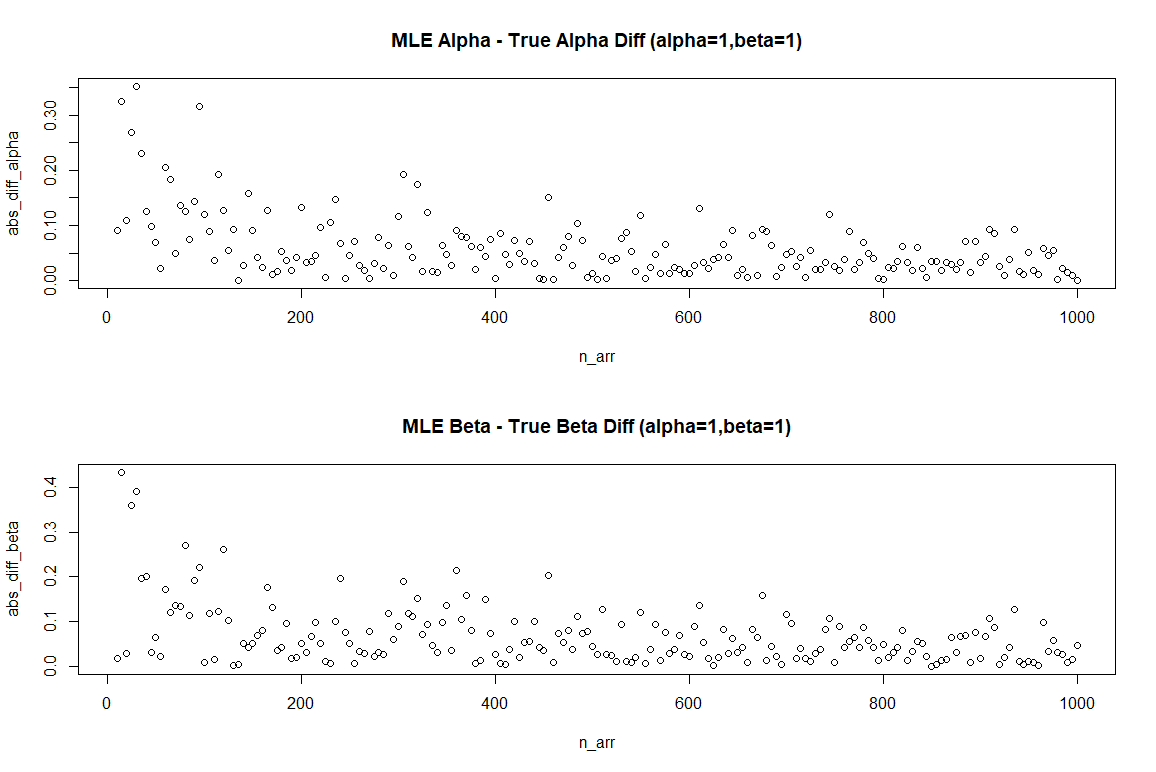
\includegraphics[scale=0.25]{abs_diff.png}
                      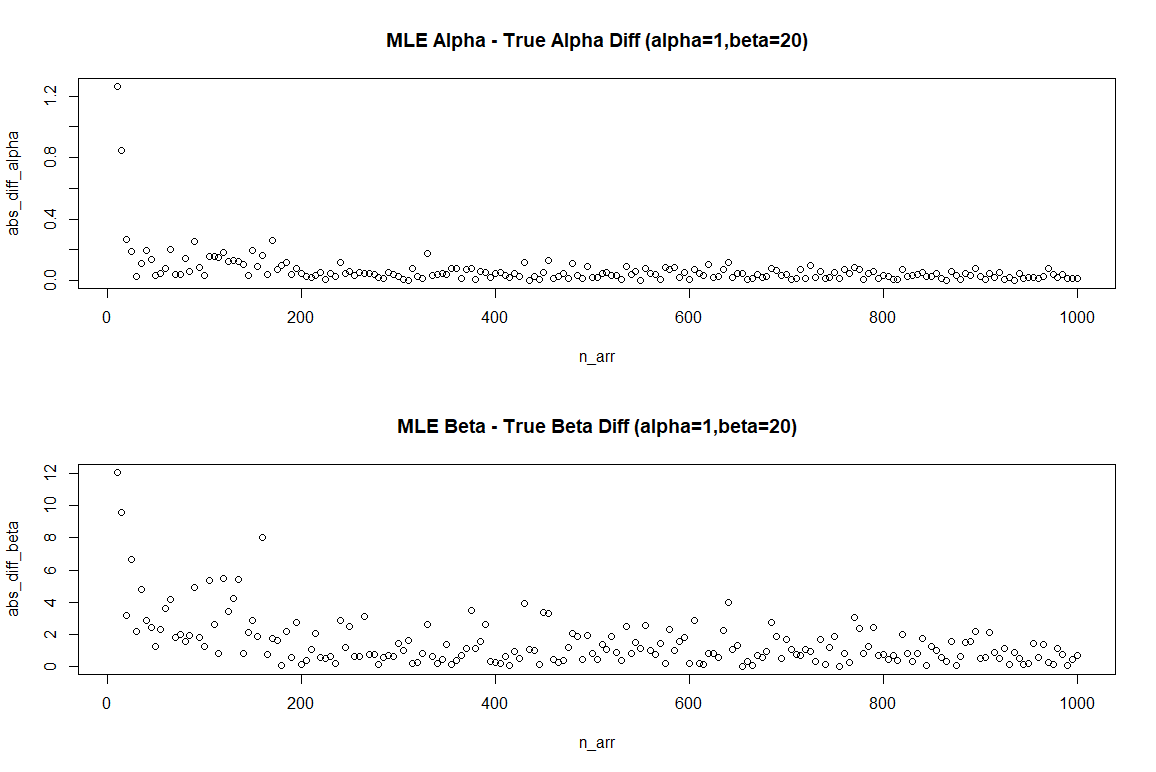
\includegraphics[scale=0.25]{abs_diff_2.png}

                      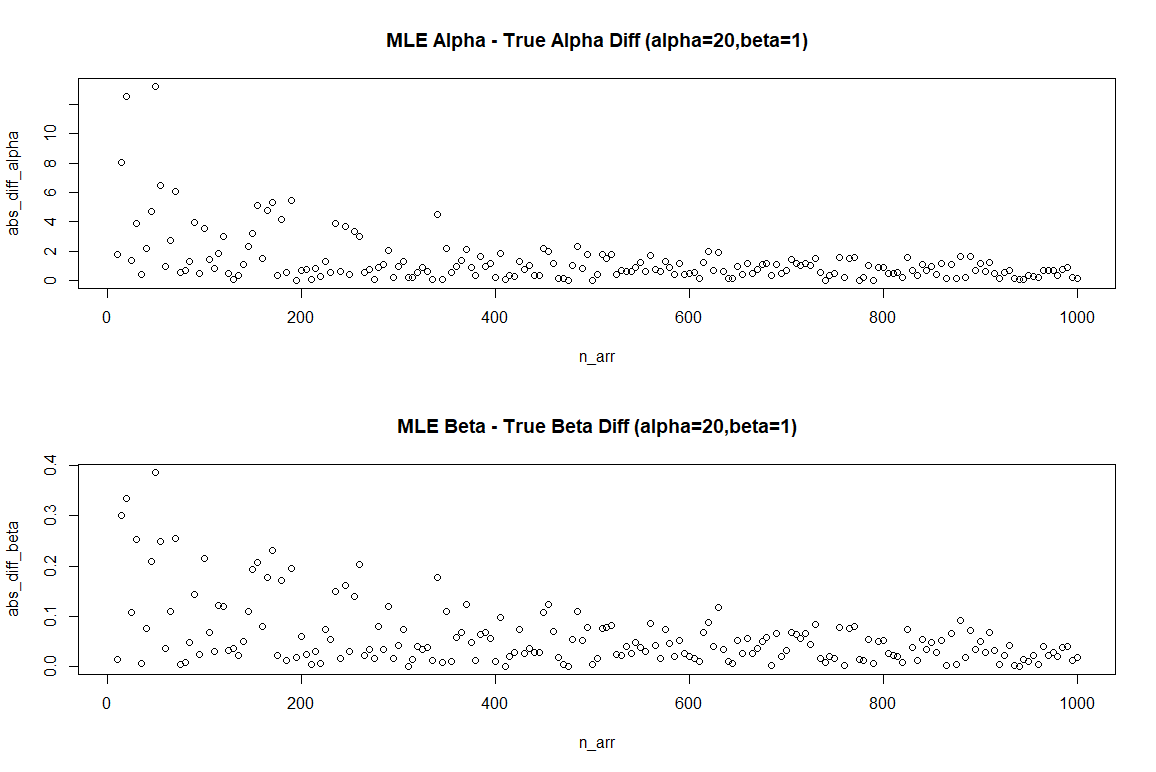
\includegraphics[scale=0.25]{abs_diff_3.png}
                      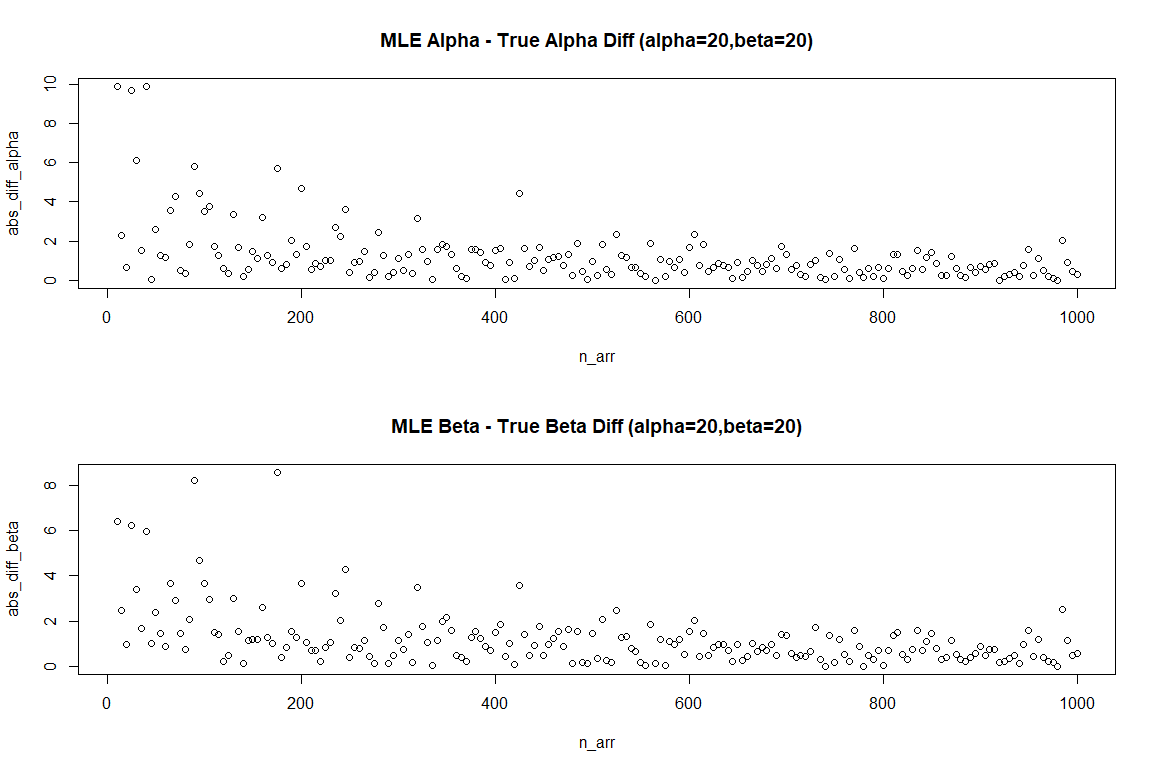
\includegraphics[scale=0.25]{abs_diff_4.png}
                  \fi


        \end{enumerate}
    \end{solution}
\end{Exercise}

\newpage
% Exercie 6
\begin{Exercise}
    \begin{solution}
        First we expand the expression
        \begin{align*}
            \sum_{i=1}^{n}(y_i - [\beta_0 + \beta_1 x_i))^2
             & = \sum_{i=1}^{n}(y_i^2 - 2(\beta_0 + \beta_1 x_i)y_i + (\beta_0^2 + 2 \beta_0 \beta_1 x_i + \beta_1^2 x_i^2))    \\
             & = \sum_{i=1}^{n}(y_i^2 - 2\beta_0 y_i - 2 \beta_1 x_i y_i + \beta_0^2 + 2 \beta_0 \beta_1 x_i + \beta_1^2 x_i^2) \\
        \end{align*}
        The minimization is found by taking partial derivative and set it to 0
        \begin{align}
            \frac{\partial}{\partial \beta_1}
            = -2\sum_{i=1}^{n} x_i y_i + 2\beta_0 \sum_{i=1}^{n} x_i + 2\beta_1 \sum_{i=1}^{n} x_i^2 & = 0 \\
            \sum_{i=1}^{n} x_i y_i - \beta_0 \sum_{i=1}^{n} x_i - \beta_1 \sum_{i=1}^{n} x_i^2       & = 0
        \end{align}

        \begin{align*}
            \frac{\partial}{\partial \beta_0}
            = -2 \sum_{i=1}^{n} y_i + 2n\beta_0  + 2\beta_1 \sum_{i=1}^{n} x_i = 0
        \end{align*}

        \[\beta_0 = \frac{\sum_{i=1}^{n} y_i - \beta_1 \sum_{i=1}^{n} x_i}{n} = \bar y - \beta_1 \bar x\]

        Now we solve this system of equation by substituting \(\beta_0\) into (2)

        \begin{align*}
            \sum_{i=1}^{n} x_i y_i - (\frac{\sum_{i=1}^{n} y_i - \beta_1 \sum_{i=1}^{n} x_i}{n}) \sum_{i=1}^{n} x_i - \beta_1 \sum_{i=1}^{n} x_i^2              & = 0 \\
            \sum_{i=1}^{n} x_i y_i - \frac{\sum_{i=1}^{n} y_i \sum_{i=1}^{n} x_i}{n} + \frac{\beta_1 (\sum_{i=1}^{n} x_i)^2}{n}  - \beta_1 \sum_{i=1}^{n} x_i^2 & = 0 \\
            \sum_{i=1}^{n} x_i y_i - \frac{\sum_{i=1}^{n} y_i \sum_{i=1}^{n} x_i}{n} + \beta_1(\frac{(\sum_{i=1}^{n} x_i)^2}{n}  - \sum_{i=1}^{n} x_i^2)        & = 0 \\
        \end{align*}
        \[\beta_1 = \frac{-\frac{1}{n} \sum_{i=1}^{n} y_i  \sum_{i=1}^{n} x_i + \sum_{i=1}^{n}  x_i y_i}{-\frac{1}{n}(\sum_{i=1}^{n} x_i)^2 + \sum_{i=1}^{n} x_i^2}\]
        Let \(r\) be the correlation between X and Y, and \(r\) is defined as the following \cite{wackerly}
        \[r = \frac{\sum_{i=1}^n (x_i - \bar x)(y_i-\bar y)}{\sqrt{\sum_{i=1}^{n} (x_i-\bar x)^2 \sum_{i=1}^{n} (y_i - \bar y)^2}}\]
        \(s_x\) are defined as\[s_x = \sqrt\frac{\sum_{i=1}^{n}  (x_i-\bar x)^2}{n-1}\]
        \(s_y\) are defined as\[s_y = \sqrt\frac{\sum_{i=1}^{n}  (y_i-\bar y)^2}{n-1}\]

        % \[\frac{s_y}{s_x} = \sqrt\frac{\sum_{i=1}^{n} (y_i - \bar y)^2}{\sum_{i=1}^{n} (x_i -\bar x)^2}\]

        % \begin{align*}
        % r\frac{s_y}{s_x} &= \frac{\sum_{i=1}^n (x_i - \bar x)(y_i-\bar y)\sum_{i=1}^{n} (y_i - \bar y)^2}{\sum_{i=1}^{n} (x_i - \bar x)^2}
        % \end{align*}

        \newpage
        Let \(S_x = \sum_{i=1}^{n}  x_i\)
        Let \(S_y = \sum_{i=1}^{n}  y_i\)
        Let \(S_{xy} = \sum_{i=1}^{n}  x_iy_i\)
        Let \(S_{xx} = \sum_{i=1}^{n}  x_i^2\)

        We then rewrite
        \[\beta_1 = \frac{S_{xy}-\frac{S_xS_y}{n}}{S_{xx}- \frac{S_x^2}{n}}\]

        and expand
        \begin{align*}
            \sum_{i=1}^{n} (x_i - \bar x)(y_i - \bar y) & = S_{xy} - (\frac{S_y}{n})S_x - (\frac{S_x}{n})S_y +\frac{(S_x S_y)}{n} \\
                                                        & = S_{xy} - \frac{S_x S_y}{n}                                            \\
                                                        & = S_{xy} - \frac{\frac{S_x S_y}{n}}{n}
        \end{align*}

        Similarly, also expand
        \[(x_i - \bar x)^2 = {S_{xx} - (\frac{S_x^2}{n})}\]
        \[(y_i - \bar y)^2 = {S_{yy} - (\frac{S_y^2}{n})}\]

        Next we rewrite \[r = \frac{S_{xy} - \frac{S_x S_y}{n}}{\sqrt{(S_{xx} - \frac{S_x^2}{n})(S_{yy} - \frac{S_y^2}{n})}}\]

        Note \[\frac{s_y}{s_x} = \frac{\sqrt{(S_{xx} - \frac{S_x^2}{n})}}{\sqrt{(S_{yy} - \frac{S_y^2}{n})}}\]

        \[r\frac{s_y}{s_x} = \beta_1 = \frac{S_{xy}-\frac{S_xS_y}{n}}{S_{xx}- \frac{S_x^2}{n}}\]
    \end{solution}
\end{Exercise}

\let \extra T

\newpage
\begin{Exercise}
    \begin{enumerate}
        \if \extra T
        \item
              \begin{minted}{r}
library(alr4)

set.seed(256) 

total_rows <- nrow(Heights)
con_set_size <- floor(total_rows / 3)
val_set_size <- total_rows - con_set_size

con_indices <- sample(seq_len(total_rows), size = con_set_size)
con_set <- Heights[con_indices, ]
val_set <- Heights[-con_indices, ]
        \end{minted}

        \item
              \begin{minted}{r}
X_train <- as.matrix(cbind(Intercept = 1, con_set$mheight))
y_train <- as.matrix(con_set$dheight)
X_val <- as.matrix(cbind(Intercept = 1, val_set$mheight))
y_val <- as.matrix(val_set$dheight)

XtX <- t(X_train) %*% X_train
XtX_inv <- solve(XtX)
Xty <- t(X_train) %*% y_train
beta <- XtX_inv %*% Xty

val_set$pred <- X_val %*% beta
val_set$resid <- val_set$dheight - val_set$pred
mse <- mean(val_set$resid^2)
rmse <- sqrt(mse)
cat(rmse) # 2.205687
        \end{minted}
        \item
              \begin{minted}{r}
resid_train <- y_train - X_train %*% beta
RSS <- sum(resid_train^2)
n <- nrow(X_train)
p <- ncol(X_train)
sigma2 <- RSS / (n - p)
X_val_XtX_inv <- X_val %*% XtX_inv
val_set$SE_pred <- sqrt(sigma2 * (1 + rowSums(X_val_XtX_inv * X_val)))
mse2 = mean(val_set$SE_pred^2)
rmse2 = sqrt(mse2)
cat(rmse2) # 2.392998
\end{minted}

              The first root average squared prediction error is only .2 lower than 2nd prediction error.

              \fi


    \end{enumerate}
\end{Exercise}

\bibliographystyle{plain} % We choose the "plain" reference style
\bibliography{refs} % Entries are in the refs.bib file
\end{document}

